\documentclass[12pt]{article}
\usepackage{geometry}                % See geometry.pdf to learn the layout options. There are lots.
\geometry{letterpaper}                   % ... or a4paper or a5paper or ... 
\usepackage{graphicx}
\usepackage{amssymb}
\usepackage{amsthm}
\usepackage{epstopdf}
\usepackage[utf8]{inputenc}
\usepackage[usenames,dvipsnames]{color}
\usepackage[table]{xcolor}
\usepackage{hyperref}
\DeclareGraphicsRule{.tif}{png}{.png}{`convert #1 `dirname #1`/`basename #1 .tif`.png}

\theoremstyle{definition}

\newtheorem{ourVersion}{ \linebreak}


\newcommand{\projectname}{Schulplaner}
\newcommand{\productname}{Education Planner}
\newcommand{\projectleader}{A. Hammash}
\newcommand{\documentstatus}{In process}
%\newcommand{\documentstatus}{Submitted}
%\newcommand{\documentstatus}{Released}
\newcommand{\version}{V. 1.0}

\begin{document}
\begin{titlepage}
\begin{flushright}

\includegraphics[scale=.5]{htlleondinglogo.png}\\
\end{flushright}

\vspace{10em}

\begin{center}
{\Huge Project Proposal} \\[3em]
{\LARGE \productname} \\[3em]
\end{center}

\begin{flushleft}
\begin{tabular}{|l|l|}
\hline
Project Name & \projectname \\ \hline
Project Leader & \projectleader \\ \hline
Document state & \documentstatus \\ \hline
Version & \version \\ \hline
\end{tabular}
\end{flushleft}

\end{titlepage}
\section*{Revisions}
\begin{tabular}{|l|l|l|}
\hline
\cellcolor[gray]{0.5}\textcolor{white}{Date} & \cellcolor[gray]{0.5}\textcolor{white}{Author} & \cellcolor[gray]{0.5}\textcolor{white}{Change} \\ \hline
October 10, 2021&H. Hajredini/ A. Hammash/ D. Fetaj&First version \\ \hline
\end{tabular}
\pagebreak

\tableofcontents
\pagebreak

\section{Introduction}

\begin{ourVersion}
Our project focusses on making it easier for students to keep track of their due dates. 
We are planning on using android studio to make this app. 
By daily reminders, an overview of the next deadline-days and also a week and month overview of the schools timetable, 
we want to get a different school planer than the usual ones. 
\end{ourVersion}
\pagebreak

\section{Initial Situation}

\begin{ourVersion}
Students already have an overview over their timetable by using Webuntis and they also can work with calendars where they can enter the next deadline-days, homework or other important things.
But by working with two or more apps one could lose the overview very easily and it also could be very annoying to continually change the app for things that could be possible to use in just one app. 
So whats missing is a easily usable app where you can work with all these features and where you have acces to all your important informations. Our app can also be used as a class-school planer where the whole class can work with one timetable. The idea is that one student can enter a homework to a subject and it will be shown to the whole class so it is comparable with substitutions of teacher. 
\end{ourVersion}
\pagebreak

\section{General Conditions and Constraints}

\begin{ourVersion}
The proposed system has to the deal with the following constraints: \linebreak

\subsection{Technical Constraints}
The app should sync with Webuntis and also a backend is necessary to store common events (for the whole class) centrally. Therefore, a dedicated server which is available via the internet has to be installed. An extra feature that might be added is the ability to insert private events in your calendar.
Further on, Webuntis, common class events and personal events have to be merged in one view which is going to be possible by saving those data on a cloud backup service. This way the user wont lose his private events in the case of losing or changing their device.

\subsection{Organisational Constraints}
Userdata, which includes the login information for webuntis and the other events that get added, has to be encrypted.
Our plan is for the app to be accessable only via mobile phone, because students use their phones to enter dates most of the time anyways. From our experience, phones are used more often throughout the day.

\end{ourVersion}

\pagebreak

\section{Project Objectives and System Concepts}

\begin{ourVersion}
The project’s use case will usually be like this: 
By opening the app the students can see first what they have to do in the next time by a pop up which covers the whole screen.
The Webuntis-Sync helps them plan their whole week or month more easily and by including the timetable, they also would have a much better overview over the canceled hours or the coming school events.

They also can enter their Homework to its respective subject and schedule.
By this, they can easily see if they have homework to do or not, and when a subject is chosen a more informative window will pop up showing exactly what the homework is.

There will be two views. The monthly-view, which will show a clearer overview of project timespans and duedates, and the weekly-view will show the timetable and the homeworks for each subject, this will be visually emphasized. 

\begin{center}
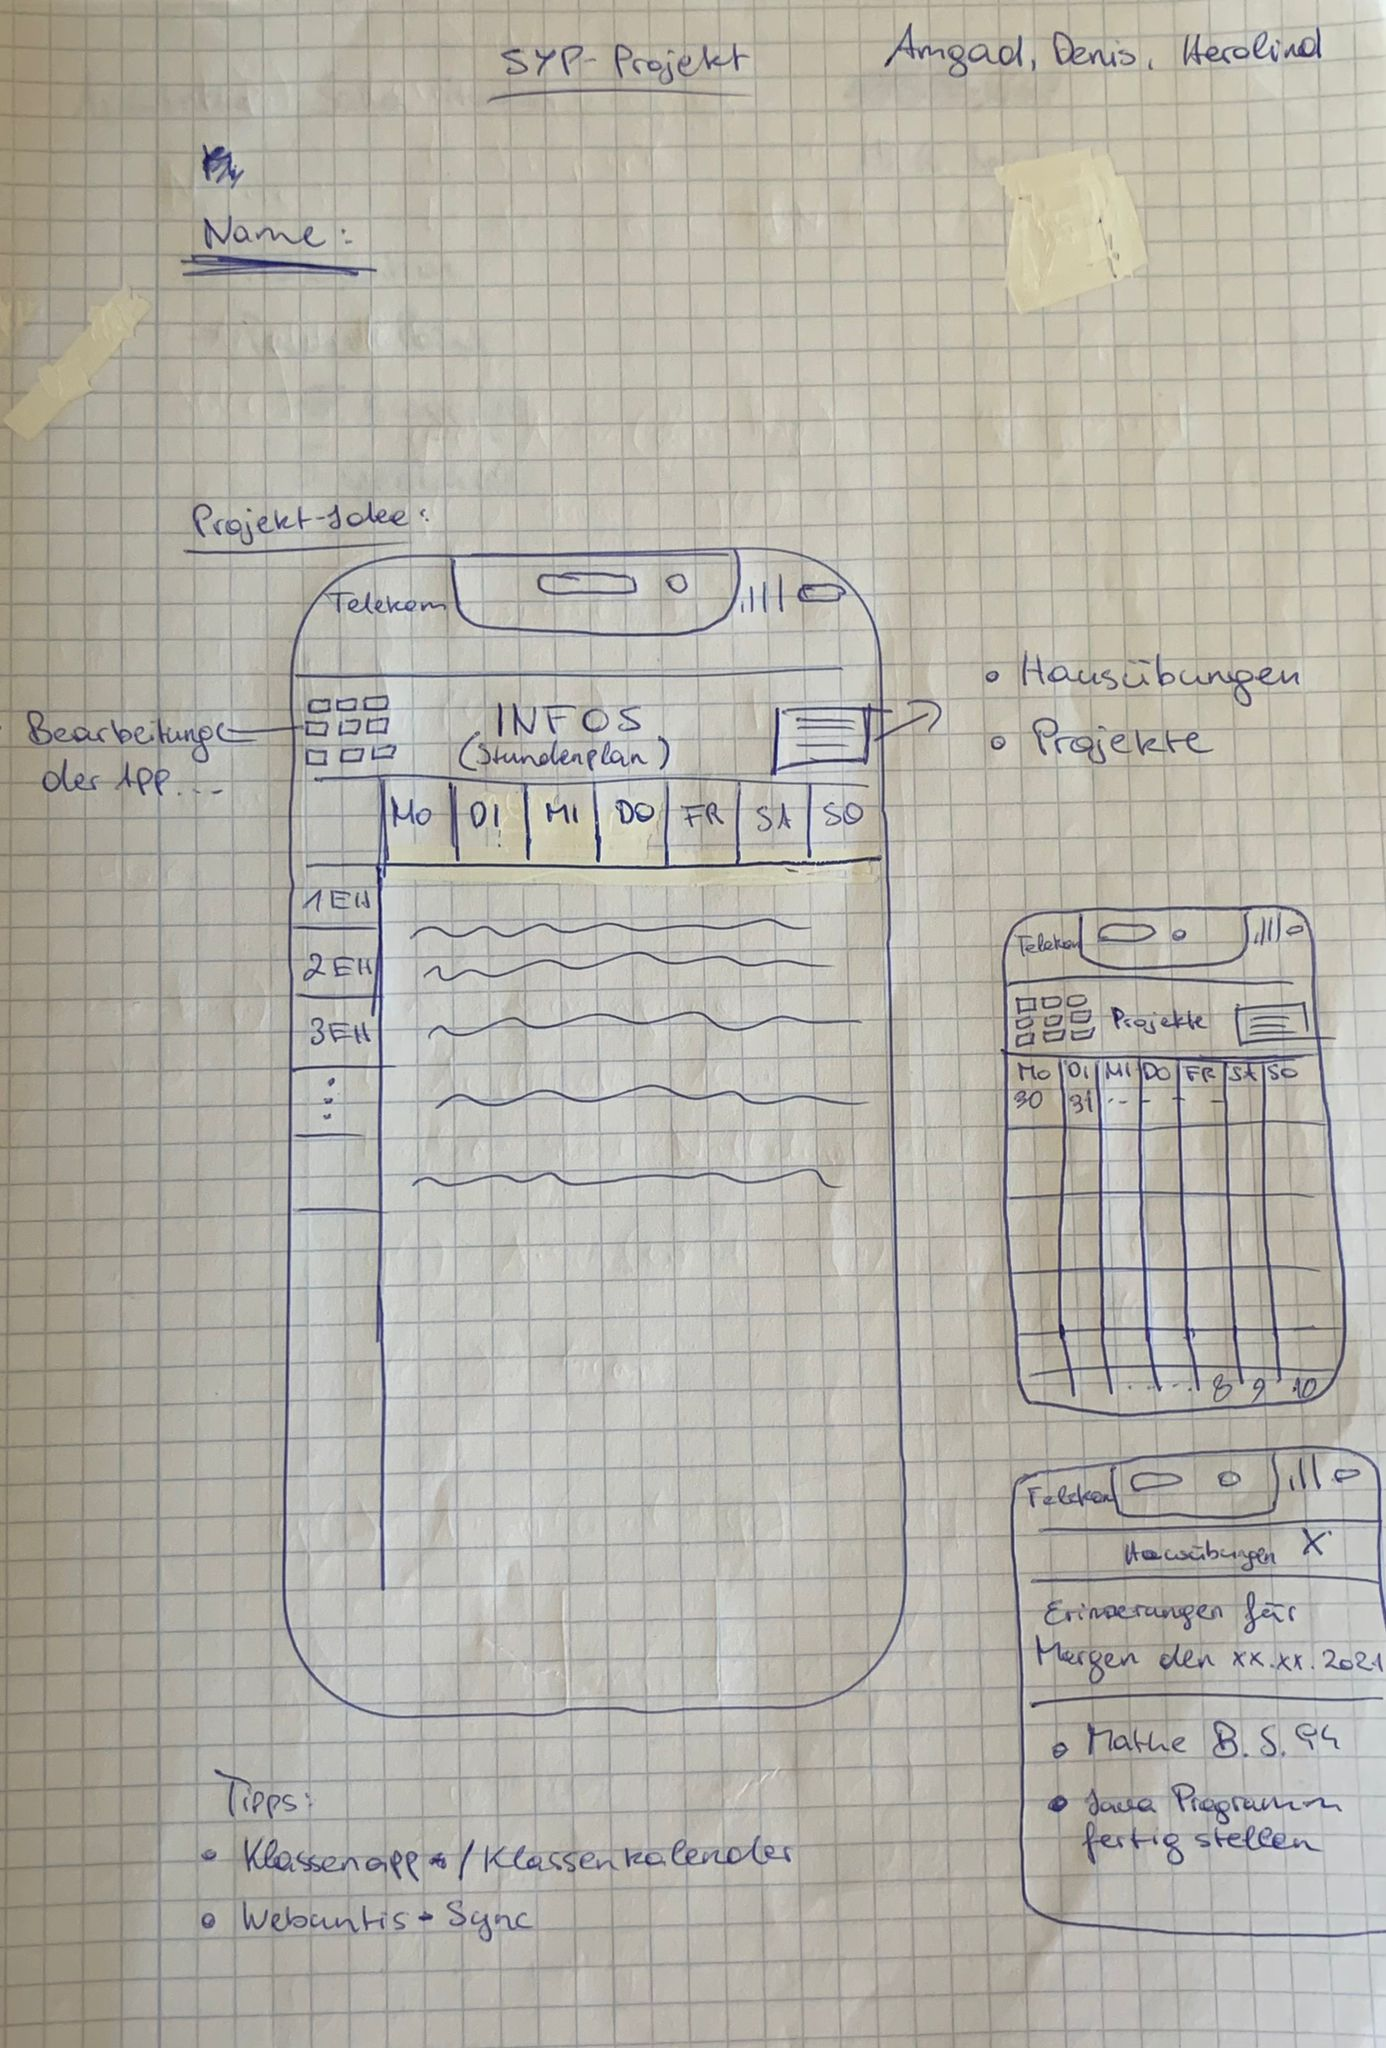
\includegraphics[scale=0.13]{AppBlueprint.jpeg}
\end{center}

\end{ourVersion}

\pagebreak
\section{Opportunities and Risks}

 \begin{ourVersion}

The project’s opportunities are:

The App will collab with companies such as Google, Apple and Amazon to make it possible for the Voice Assistants to enter appointment dates easily via voice commands. 
This allows the app to not only be usefull for students, but for busy people too, because it can also save shopping lists, making it helpful for adults too.
An easy, straight forward to use app that mixes Notes, Calender and School and/or Work timetable.

Risks to consider: 
If webuntis gets outdated too soon this app won't have the chance to take off and develop.
The cloud server the data is save in may crash or outright stop their service, forcing us to make our own server which is at the moment not possible.
Webuntis and other partaking companies may deny our offer, resulting in big problems, depending what role the company plays in our app.
	
 \end{ourVersion}


\pagebreak

\section{Milestones}
\begin{ourVersion}
\begin{center}
\begin{tabular}{||c c c||}
 \hline
 Milestones & Status & Start date \\ [0.5ex] 
 \hline\hline
 Finding and getting comfortable with the working environment  & Running... & February 2022 \\ 
 \hline   
 First visual impession of app & Ready & February 2022 \\
 \hline
 save user input dates & Blocked & March 2022 \\
 \hline
 Sync with webuntis & Blocked & July 2022 \\
 \hline
 Saving Notes and Grocery Lists & Blocked & October 2022\\
 \hline
 Finilzing and refining the app & Blocked & Unknown \\ [1ex] 
 \hline 

\end{tabular}
\end{center}
\end{ourVersion}


\pagebreak

\section{Planning}

\begin{ourVersion}
We plan on having the app show a synced-up week view from Webuntis and have it be interactable 
so students can already write their homework on it, that will be our first mile-stone. 
The roles of the team members will be that same and we’ll divide the workload be-tween us. 
The app will be made in Android studio and the files may have to be saved lo-cally.
\end{ourVersion}

\end{document}  